\documentclass[border=4pt,convert={density=800,size=600x600,outext=.png}]{standalone}
\usepackage{tikz}
\begin{document}
% first method
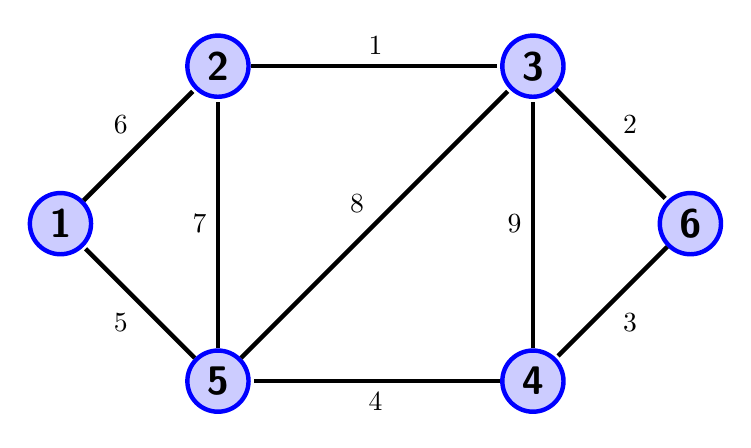
\begin{tikzpicture}[shorten >=1pt, auto, node distance=3cm, ultra thick,
   node_style/.style={circle,draw=blue,fill=blue!20!,font=\sffamily\Large\bfseries},
   edge_style/.style={draw=black, ultra thick}]
    \node[node_style] (v1) at (-2,2) {2};
    \node[node_style] (v2) at (2,2) {3};
    \node[node_style] (v3) at (4,0) {6};
    \node[node_style] (v4) at (2,-2) {4};
    \node[node_style] (v5) at (-2,-2) {5};
    \node[node_style] (v6) at (-4,0) {1};
    \draw[edge_style]  (v1) edge node{1} (v2);
    \draw[edge_style]  (v2) edge node{2} (v3);
    \draw[edge_style]  (v3) edge node{3} (v4);
    \draw[edge_style]  (v4) edge node{4} (v5);
    \draw[edge_style]  (v5) edge node{5} (v6);
    \draw[edge_style]  (v6) edge node{6} (v1);
    \draw[edge_style]  (v5) edge node{7} (v1);
    \draw[edge_style]  (v5) edge node{8} (v2);
    \draw[edge_style]  (v4) edge node{9} (v2);
\end{tikzpicture}
\end{document}
